\section{CƠ SỞ LÝ THUYẾT}

\subsection{Tổng quan về học tăng cường}

Học tăng cường (reinforcement learning -- RL) nghiên cứu cách một tác tử lựa chọn hành động khi tương tác với môi trường để tối đa hóa phần thưởng tích lũy. Khác với học có giám sát, tác tử không nhận sẵn nhãn cho từng quyết định. Thay vào đó, tác tử quan sát kết quả của các hành động đã thực hiện và điều chỉnh cách ra quyết định dựa trên phần thưởng nhận được. Bốn thành phần cơ bản của một hệ thống RL gồm chính sách, tín hiệu phần thưởng, hàm giá trị và mô hình môi trường nếu mô hình đó được biết hoặc được học \cite{SuttonBarto2018,TranDinhTanAICourse}.

Trong phạm vi đề tài, ba thuật toán Q-Learning, DQN và Double DQN đều thuộc nhóm phương pháp dựa trên giá trị (value-based methods). Các phương pháp này học giá trị của hành động trong từng trạng thái, sau đó ưu tiên hành động có giá trị ước lượng lớn nhất. Điểm khác biệt chính nằm ở cách biểu diễn giá trị hành động và cách xây dựng giá trị mục tiêu trong quá trình cập nhật.

\subsubsection{Quá trình quyết định Markov}

Quá trình quyết định Markov (Markov Decision Process -- MDP) là mô hình toán học cho bài toán ra quyết định tuần tự. Tại thời điểm $t$, tác tử nhận trạng thái $S_t \in \mathcal{S}$, lựa chọn hành động $A_t \in \mathcal{A}(S_t)$, sau đó môi trường trả về phần thưởng $R_{t+1}$ và trạng thái tiếp theo $S_{t+1}$. Chuỗi tương tác có dạng
\begin{equation}
    S_0, A_0, R_1, S_1, A_1, R_2, S_2, \ldots
    \label{eq:mdp-trajectory}
\end{equation}

Mối quan hệ giữa tác tử và môi trường được minh họa trong \figref{fig:agent-environment}. Hành động đi từ tác tử tới môi trường, còn trạng thái và phần thưởng đi theo chiều ngược lại.

\begin{figure}[H]
    \centering
    \begin{tikzpicture}[
        component/.style={
            draw,
            rounded corners=2pt,
            minimum width=4.0cm,
            minimum height=1.35cm,
            align=center,
            fill=black!4
        },
        flow/.style={-{Latex[length=2.5mm]}, thick}
    ]
        \node[component] (agent) {Tác tử};
        \node[component, right=5.0cm of agent] (environment) {Môi trường};

        \draw[flow]
            ([yshift=7pt]agent.east)
            --
            node[above]{Hành động $A_t$}
            ([yshift=7pt]environment.west);

        \draw[flow]
            ([yshift=-7pt]environment.west)
            --
            node[below, align=center]{Phần thưởng $R_{t+1}$\\Trạng thái $S_{t+1}$}
            ([yshift=-7pt]agent.east);
    \end{tikzpicture}
    \caption{Tương tác giữa tác tử và môi trường trong MDP \cite{SuttonBarto2018}.}
    \label{fig:agent-environment}
\end{figure}

Với MDP hữu hạn, động lực của môi trường có thể được mô tả bằng phân phối xác suất
\begin{equation}
    p(s',r \mid s,a)
    =
    \Pr\!\left\{
        S_{t+1}=s',\,R_{t+1}=r
        \mid
        S_t=s,\,A_t=a
    \right\}.
    \label{eq:mdp-dynamics}
\end{equation}
Phân phối này cho biết xác suất chuyển tới trạng thái $s'$ và nhận phần thưởng $r$ khi tác tử thực hiện hành động $a$ tại trạng thái $s$. Tính chất Markov yêu cầu trạng thái hiện tại phải chứa những thông tin từ quá khứ có ảnh hưởng đến diễn biến tương lai. Khi đã biết $S_t$ và $A_t$, xác suất của trạng thái cùng phần thưởng tiếp theo không phụ thuộc thêm vào toàn bộ lịch sử trước đó \cite{SuttonBarto2018}.

Một chính sách (policy) được ký hiệu bởi $\pi(a \mid s)$, biểu diễn xác suất lựa chọn hành động $a$ tại trạng thái $s$. Mục tiêu của tác tử là tìm chính sách tạo ra phần thưởng tích lũy kỳ vọng lớn. Đối với bài toán theo episode như Mini Pacman, mỗi episode kết thúc khi tác tử đạt điều kiện kết thúc của môi trường hoặc chạm giới hạn số bước.

\subsubsection{Phần thưởng tích lũy và hàm giá trị}

Phần thưởng tức thời chỉ phản ánh kết quả ngay sau một hành động. Để đánh giá ảnh hưởng dài hạn, RL sử dụng phần thưởng tích lũy có chiết khấu, còn gọi là return. Tại thời điểm $t$, return được định nghĩa là
\begin{equation}
    G_t
    =
    R_{t+1}
    + \gamma R_{t+2}
    + \gamma^2 R_{t+3}
    + \cdots
    =
    \sum_{k=0}^{\infty}\gamma^k R_{t+k+1},
    \label{eq:discounted-return}
\end{equation}
trong đó $\gamma \in [0,1]$ là discount factor. Giá trị $\gamma$ nhỏ làm tác tử ưu tiên phần thưởng gần, còn giá trị gần $1$ làm tăng ảnh hưởng của phần thưởng trong tương lai. Với bài toán theo episode, tổng trên kết thúc tại trạng thái terminal và giá trị sau thời điểm kết thúc được xem bằng $0$ \cite{SuttonBarto2018}.

Hàm giá trị trạng thái dưới chính sách $\pi$ được định nghĩa bởi
\begin{equation}
    v_{\pi}(s)
    =
    \mathbb{E}_{\pi}\!\left[G_t \mid S_t=s\right].
    \label{eq:state-value}
\end{equation}
Đại lượng này cho biết return kỳ vọng khi bắt đầu tại trạng thái $s$ và tiếp tục lựa chọn hành động theo $\pi$. Tương tự, hàm giá trị hành động là
\begin{equation}
    q_{\pi}(s,a)
    =
    \mathbb{E}_{\pi}\!\left[G_t \mid S_t=s, A_t=a\right],
    \label{eq:action-value}
\end{equation}
cho biết return kỳ vọng khi chọn hành động $a$ tại $s$, sau đó tiếp tục theo chính sách $\pi$.

Giá trị hành động tối ưu được ký hiệu là
\begin{equation}
    q_{*}(s,a)
    =
    \max_{\pi} q_{\pi}(s,a).
    \label{eq:optimal-action-value}
\end{equation}
Hàm này thỏa mãn phương trình tối ưu Bellman
\begin{equation}
    q_{*}(s,a)
    =
    \sum_{s',r}
    p(s',r \mid s,a)
    \left[
        r + \gamma \max_{a'} q_{*}(s',a')
    \right].
    \label{eq:bellman-optimality}
\end{equation}
Phương trình~\eqref{eq:bellman-optimality} là cơ sở của các thuật toán học giá trị. Giá trị của một cặp trạng thái--hành động được liên hệ với phần thưởng tức thời và giá trị tốt nhất có thể đạt được ở trạng thái tiếp theo \cite{SuttonBarto2018}.

\subsubsection{Khám phá và khai thác}

Trong quá trình học, tác tử phải cân bằng giữa khám phá (exploration) và khai thác (exploitation). Khai thác chọn hành động đang có Q-value lớn nhất, còn khám phá thử các hành động khác để thu thập thêm kinh nghiệm. Nếu chỉ khai thác từ đầu, tác tử có thể duy trì một hành động chưa thực sự tối ưu do các Q-value ban đầu còn thiếu chính xác. Nếu khám phá quá nhiều, tác tử không tận dụng được những gì đã học.

Một chiến lược phổ biến là $\epsilon$-greedy. Giả sử tại trạng thái $s$ chỉ có một hành động tham lam
\begin{equation}
    a^{*}
    =
    \underset{a' \in \mathcal{A}(s)}{\arg\max}\,Q(s,a').
    \label{eq:greedy-action}
\end{equation}
Xác suất lựa chọn hành động được xác định bởi
\begin{equation}
    \pi_{\epsilon}(a \mid s)
    =
    \begin{cases}
        1-\epsilon+\dfrac{\epsilon}{|\mathcal{A}(s)|},
        & \text{nếu } a=a^{*},\\[6pt]
        \dfrac{\epsilon}{|\mathcal{A}(s)|},
        & \text{nếu } a\neq a^{*}.
    \end{cases}
    \label{eq:epsilon-greedy}
\end{equation}
Với xác suất $1-\epsilon$, tác tử chọn hành động tham lam. Với xác suất $\epsilon$, tác tử chọn ngẫu nhiên trong tập hành động, vì vậy hành động tham lam vẫn có thể được chọn trong nhánh ngẫu nhiên. Trong thực nghiệm, $\epsilon$ thường giảm dần để ưu tiên khám phá ở giai đoạn đầu và khai thác nhiều hơn khi các Q-value đã ổn định hơn \cite{SuttonBarto2018}.

\subsection{Q-Learning}

Q-Learning được sử dụng trong đề tài như một phương pháp học dạng bảng. Thuật toán lưu Q-value của từng cặp trạng thái--hành động trong Q-table và cập nhật giá trị này từ phần thưởng cùng giá trị tốt nhất tại trạng thái tiếp theo. Q-Learning là phương pháp temporal-difference control không cần mô hình môi trường và thuộc nhóm off-policy: hành động tạo dữ liệu có thể được chọn bằng $\epsilon$-greedy, trong khi target sử dụng hành động có Q-value lớn nhất \cite{WatkinsDayan1992,SuttonBarto2018}.

Sau khi tác tử thực hiện $A_t$ tại $S_t$, nhận $R_{t+1}$ và chuyển tới $S_{t+1}$, phần tử tương ứng trong Q-table được cập nhật theo
\begin{equation}
    \begin{aligned}
    Q_{t+1}(S_t,A_t)
    =
    Q_t(S_t,A_t)
    + \alpha
    \Big[
        R_{t+1}
        + \gamma \max_{a'}Q_t(S_{t+1},a')
        - Q_t(S_t,A_t)
    \Big],
    \end{aligned}
    \label{eq:q-learning-update}
\end{equation}
trong đó $\alpha \in (0,1]$ là learning rate. Các phần tử khác của Q-table không thay đổi tại bước cập nhật này. Nếu $S_{t+1}$ là trạng thái terminal, thành phần giá trị tương lai được đặt bằng $0$.

Giá trị mục tiêu của cập nhật có thể viết là
\begin{equation}
    Y_t^{\mathrm{Q}}
    =
    R_{t+1}
    + \gamma \max_{a'}Q_t(S_{t+1},a'),
    \label{eq:q-learning-target}
\end{equation}
và sai số temporal difference là
\begin{equation}
    \delta_t
    =
    Y_t^{\mathrm{Q}}-Q_t(S_t,A_t).
    \label{eq:q-learning-td-error}
\end{equation}
Như vậy, Q-Learning dịch chuyển Q-value hiện tại một đoạn bằng $\alpha\delta_t$ về phía giá trị mục tiêu.

Quy trình của một bước Q-Learning gồm:
\begin{enumerate}
    \item Quan sát trạng thái hiện tại $S_t$.
    \item Chọn hành động $A_t$, thường bằng chiến lược $\epsilon$-greedy.
    \item Thực hiện hành động và nhận $R_{t+1}$ cùng $S_{t+1}$.
    \item Tính target theo phương trình~\eqref{eq:q-learning-target}.
    \item Cập nhật phần tử $Q(S_t,A_t)$ theo phương trình~\eqref{eq:q-learning-update}.
\end{enumerate}

Quy trình trên được minh họa trong \figref{fig:q-learning-principle}. Hình nhấn mạnh rằng mỗi bước chỉ cập nhật phần tử Q-value tương ứng với cặp trạng thái--hành động vừa quan sát.

\begin{figure}[H]
    \centering
    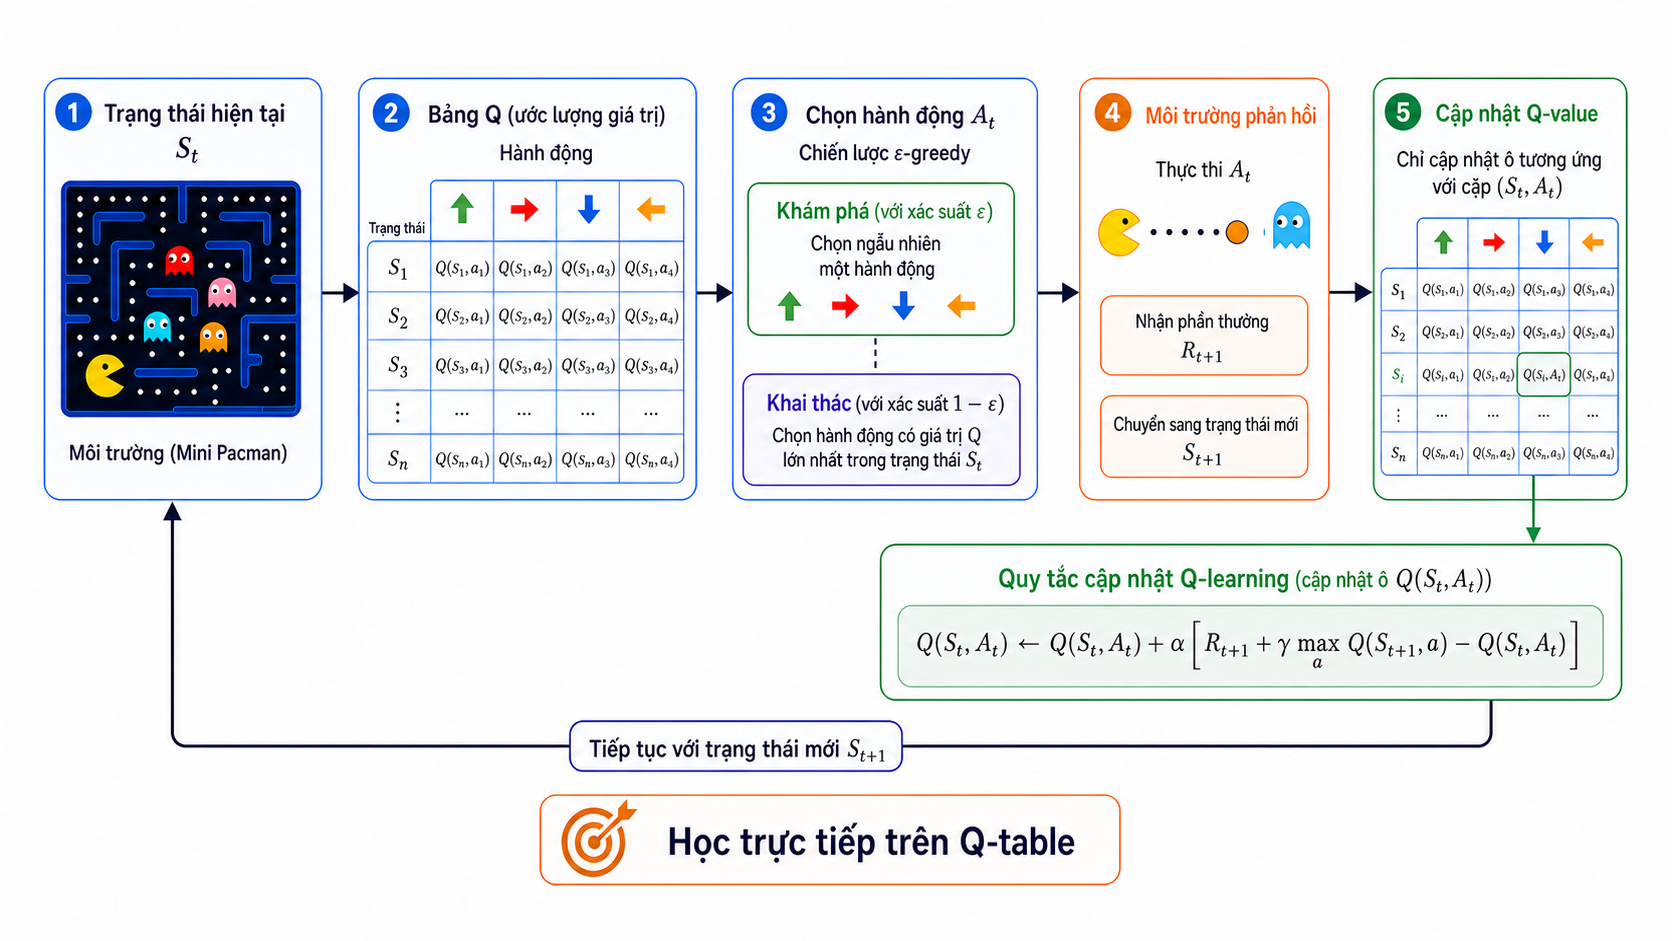
\includegraphics[width=\textwidth]{image/q_learning_principle.png}
    \caption{Quy trình lựa chọn hành động và cập nhật Q-table của Q-Learning \cite{WatkinsDayan1992,SuttonBarto2018}.}
    \label{fig:q-learning-principle}
\end{figure}

Về mặt lý thuyết, Q-Learning có thể hội tụ về action-value tối ưu với xác suất $1$ khi mọi cặp trạng thái--hành động tiếp tục được lấy mẫu và dãy learning rate thỏa mãn các điều kiện xấp xỉ ngẫu nhiên phù hợp \cite{WatkinsDayan1992}. Kết quả này không bảo đảm rằng mọi quá trình huấn luyện hữu hạn với learning rate cố định đều hội tụ.

Q-table giúp quy trình cập nhật dễ theo dõi nhưng phải lưu riêng Q-value cho từng cặp trạng thái--hành động. Khi số trạng thái tăng, kích thước bảng lớn hơn và các trạng thái khác nhau không có cơ chế chia sẻ thông tin. DQN xử lý hạn chế này bằng cách sử dụng mạng nơ-ron để xấp xỉ Q-value.

\subsection{Deep Q-Network}

Deep Q-Network (DQN) mở rộng Q-Learning bằng cách sử dụng mạng nơ-ron để xấp xỉ hàm giá trị hành động thay cho Q-table. Quá trình huấn luyện kết hợp experience replay nhằm tái sử dụng các chuyển tiếp và target network nhằm giữ giá trị mục tiêu ổn định hơn \cite{Mnih2013,Mnih2015}.

\subsubsection{Mạng Q}

Thay vì lưu một Q-table, DQN sử dụng mạng nơ-ron có tham số $\theta$ để xấp xỉ
\begin{equation}
    Q(s,a;\theta)
    \approx
    q_{*}(s,a).
    \label{eq:q-network-approximation}
\end{equation}
Với một trạng thái đầu vào, mạng Q xuất ra vector giá trị
\begin{equation}
    \mathbf{Q}(s;\theta)
    =
    \left[
        Q(s,a_1;\theta),
        Q(s,a_2;\theta),
        \ldots,
        Q(s,a_m;\theta)
    \right],
    \label{eq:q-network-output}
\end{equation}
trong đó $m$ là số hành động. Khi khai thác, tác tử chọn hành động có phần tử đầu ra lớn nhất. Trong quá trình khám phá, hành động vẫn được chọn theo chính sách $\epsilon$-greedy.

Q-network có thể nhận nhiều dạng biểu diễn trạng thái khác nhau. Trong đề tài, đầu vào của mạng là vector đặc trưng được xây dựng từ trạng thái Mini Pacman, không phải chuỗi khung hình như cấu hình Atari \cite{Mnih2013,Mnih2015}.

Do các trạng thái dùng chung tham số $\theta$, một lần cập nhật có thể làm thay đổi Q-value ước lượng của nhiều trạng thái. Điều này tạo khả năng khái quát hóa mà Q-table không có sẵn, nhưng cũng khiến target thay đổi trong quá trình học và có thể làm huấn luyện mất ổn định. DQN sử dụng experience replay và target network để giảm các vấn đề này.

\subsubsection{Experience replay}

Tại mỗi bước, tác tử thu được một chuyển tiếp
\begin{equation}
    e_t
    =
    (S_t,A_t,R_{t+1},S_{t+1}).
    \label{eq:transition}
\end{equation}
Các chuyển tiếp được lưu trong replay buffer $\mathcal{D}$. Khi cập nhật mạng, DQN không chỉ sử dụng chuyển tiếp mới nhất mà lấy ngẫu nhiên một mini-batch từ buffer. Với bài toán theo episode, cài đặt thực tế thường lưu thêm cờ kết thúc để xác định target có chứa giá trị tương lai hay không.

Experience replay có ba vai trò chính. Thứ nhất, một chuyển tiếp có thể được tái sử dụng trong nhiều lần cập nhật, giúp sử dụng dữ liệu hiệu quả hơn. Thứ hai, lấy mẫu ngẫu nhiên làm giảm tương quan mạnh giữa các chuyển tiếp liên tiếp. Thứ ba, dữ liệu trong buffer được tạo bởi nhiều phiên bản chính sách ở các thời điểm khác nhau, giúp làm mượt sự thay đổi của phân phối huấn luyện \cite{Mnih2013,Mnih2015}.

Replay buffer có dung lượng hữu hạn nên các chuyển tiếp cũ sẽ bị thay thế. Trong phạm vi đề tài, các chuyển tiếp được lấy mẫu đều từ buffer. Prioritized experience replay không được xem xét.

\subsubsection{Target network và loss}

DQN duy trì hai mạng có cùng kiến trúc:
\begin{itemize}
    \item Online network với tham số $\theta$ được cập nhật bằng gradient descent.
    \item Target network với tham số $\theta^{-}$ được dùng để tính giá trị mục tiêu.
\end{itemize}
Sau một số bước cập nhật cố định, tham số của online network được sao chép sang target network. Giữa hai lần đồng bộ, $\theta^{-}$ được giữ nguyên. Nhờ đó, target không thay đổi ngay sau từng lần cập nhật online network, làm giảm vòng phản hồi có thể gây dao động hoặc phân kỳ \cite{Mnih2015}.

Với một chuyển tiếp, target của DQN được xác định bởi
\begin{equation}
    Y_t^{\mathrm{DQN}}
    =
    \begin{cases}
        R_{t+1},
        & \text{nếu } S_{t+1} \text{ là terminal},\\[4pt]
        R_{t+1}
        + \gamma
        \displaystyle\max_{a'}
        Q(S_{t+1},a';\theta^{-}),
        & \text{trường hợp còn lại}.
    \end{cases}
    \label{eq:dqn-target}
\end{equation}
Online network tạo ra giá trị hiện tại $Q(S_t,A_t;\theta)$, còn target network tạo thành phần giá trị ở trạng thái tiếp theo.

Trong cài đặt của đề tài, online network được tối ưu bằng Smooth L1 Loss với ngưỡng chuyển tiếp bằng $1$. Gọi $\delta_i$ là TD error của mẫu thứ $i$, loss được xác định bởi
\begin{equation}
    \begin{aligned}
        \delta_i
        &=Y_i^{\mathrm{DQN}}-Q(s,a;\theta_i),\\
        L_i(\theta_i)
        &=\mathbb{E}_{(s,a,r,s')\sim U(\mathcal{D})}
        \left[\ell(\delta_i)\right],\\
        \ell(\delta)
        &=
        \begin{cases}
            \dfrac{1}{2}\delta^2, & \text{nếu } |\delta|<1,\\[4pt]
            |\delta|-\dfrac{1}{2}, & \text{trường hợp còn lại}.
        \end{cases}
    \end{aligned}
    \label{eq:dqn-loss}
\end{equation}
So với bình phương TD error, Smooth L1 Loss vẫn phạt sai lệch nhỏ theo dạng bậc hai nhưng chuyển sang dạng tuyến tính khi sai lệch lớn. Cách tính này đúng với hàm \texttt{SmoothL1Loss} được sử dụng trong mã nguồn của đề tài \cite{DRLPacmanGitHub}.
Learning rate của optimizer điều khiển độ lớn bước cập nhật tham số $\theta$ của online network khi tối ưu loss.

Luồng dữ liệu huấn luyện DQN được tổng hợp trong \figref{fig:dqn-training-flow}. Online network được cập nhật qua loss, còn target network chỉ nhận tham số qua bước đồng bộ định kỳ.

\begin{figure}[H]
    \centering
    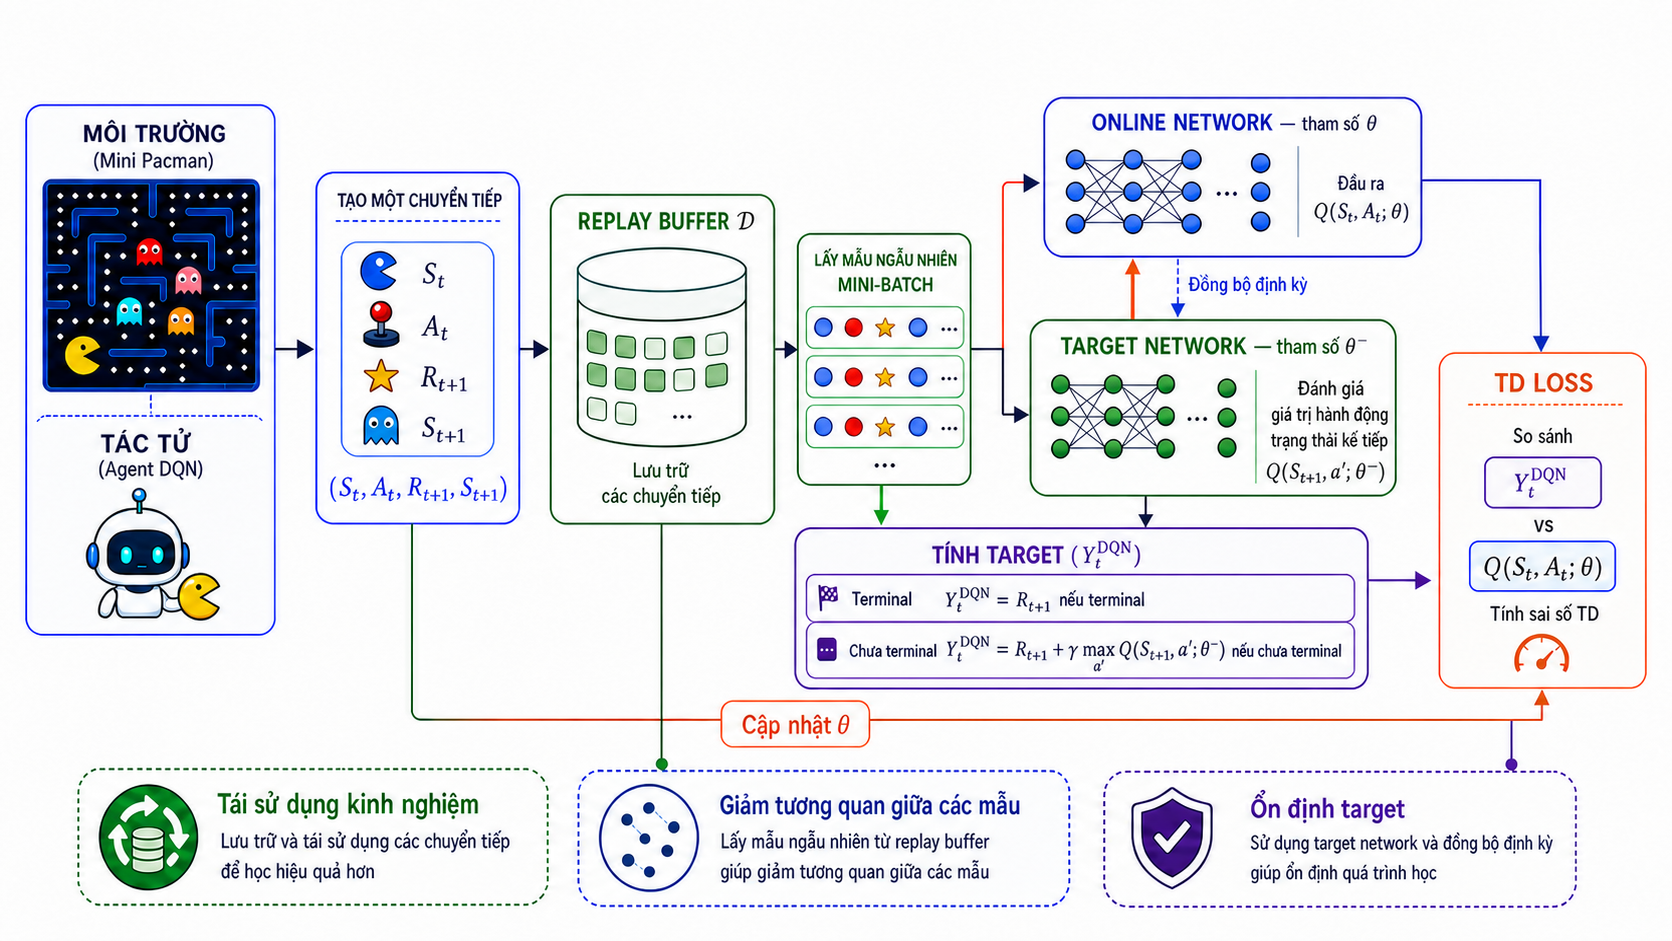
\includegraphics[width=\textwidth]{image/dqn_training_flow.png}
    \caption{Luồng huấn luyện DQN với experience replay và target network \cite{Mnih2013,Mnih2015}.}
    \label{fig:dqn-training-flow}
\end{figure}

\subsection{Double DQN}

Target của DQN trong phương trình~\eqref{eq:dqn-target} sử dụng cùng các giá trị do target network sinh ra để vừa chọn hành động có giá trị lớn nhất, vừa đánh giá hành động đó. Khi các Q-value chỉ là ước lượng và chứa sai số, phép lấy maximum có xu hướng ưu tiên những hành động đang bị đánh giá cao hơn giá trị thực. Hiện tượng này được gọi là overestimation \cite{VanHasselt2016}.

Đối với chuyển tiếp không kết thúc episode, target DQN có thể viết lại thành
\begin{equation}
    Y_t^{\mathrm{DQN}}
    =
    R_{t+1}
    +
    \gamma
    Q\!\left(
        S_{t+1},
        \underset{a'}{\arg\max}\,
        Q(S_{t+1},a';\theta_t^{-});
        \theta_t^{-}
    \right).
    \label{eq:dqn-target-expanded}
\end{equation}
Cả lựa chọn và đánh giá hành động đều dựa trên tham số $\theta_t^{-}$.

Double DQN tách hai vai trò này. Online network chọn hành động tham lam
\begin{equation}
    a_{t+1}^{*}
    =
    \underset{a'}{\arg\max}\,
    Q(S_{t+1},a';\theta_t),
    \label{eq:ddqn-action-selection}
\end{equation}
sau đó target network đánh giá hành động đã chọn. Target Double DQN là
\begin{equation}
    Y_t^{\mathrm{DDQN}}
    =
    \begin{cases}
        R_{t+1},
        & \text{nếu } S_{t+1} \text{ là terminal},\\[4pt]
        R_{t+1}
        + \gamma
        Q\!\left(
            S_{t+1},
            a_{t+1}^{*};
            \theta_t^{-}
        \right),
        & \text{trường hợp còn lại}.
    \end{cases}
    \label{eq:ddqn-target}
\end{equation}

Loss của Double DQN giữ nguyên dạng của phương trình~\eqref{eq:dqn-loss}, nhưng $Y_i^{\mathrm{DQN}}$ được thay bằng $Y_i^{\mathrm{DDQN}}$ khi tính TD error \cite{VanHasselt2016}.

Sự khác biệt nằm ở thành phần target. DQN lấy maximum trực tiếp từ target network, còn Double DQN dùng online network để chọn hành động và target network để đánh giá. Target network vẫn được đồng bộ định kỳ, còn optimizer và learning rate được giữ nguyên như DQN. Vì vậy, Double DQN không cần thêm mạng thứ ba và giữ nguyên phần còn lại của quy trình huấn luyện \cite{VanHasselt2016}.

Nguyên lý tách vai trò của Double DQN được minh họa trong \figref{fig:ddqn-selection-evaluation}. Online network chọn hành động tham lam tại trạng thái tiếp theo, còn target network đánh giá chính hành động đã chọn.

\begin{figure}[H]
    \centering
    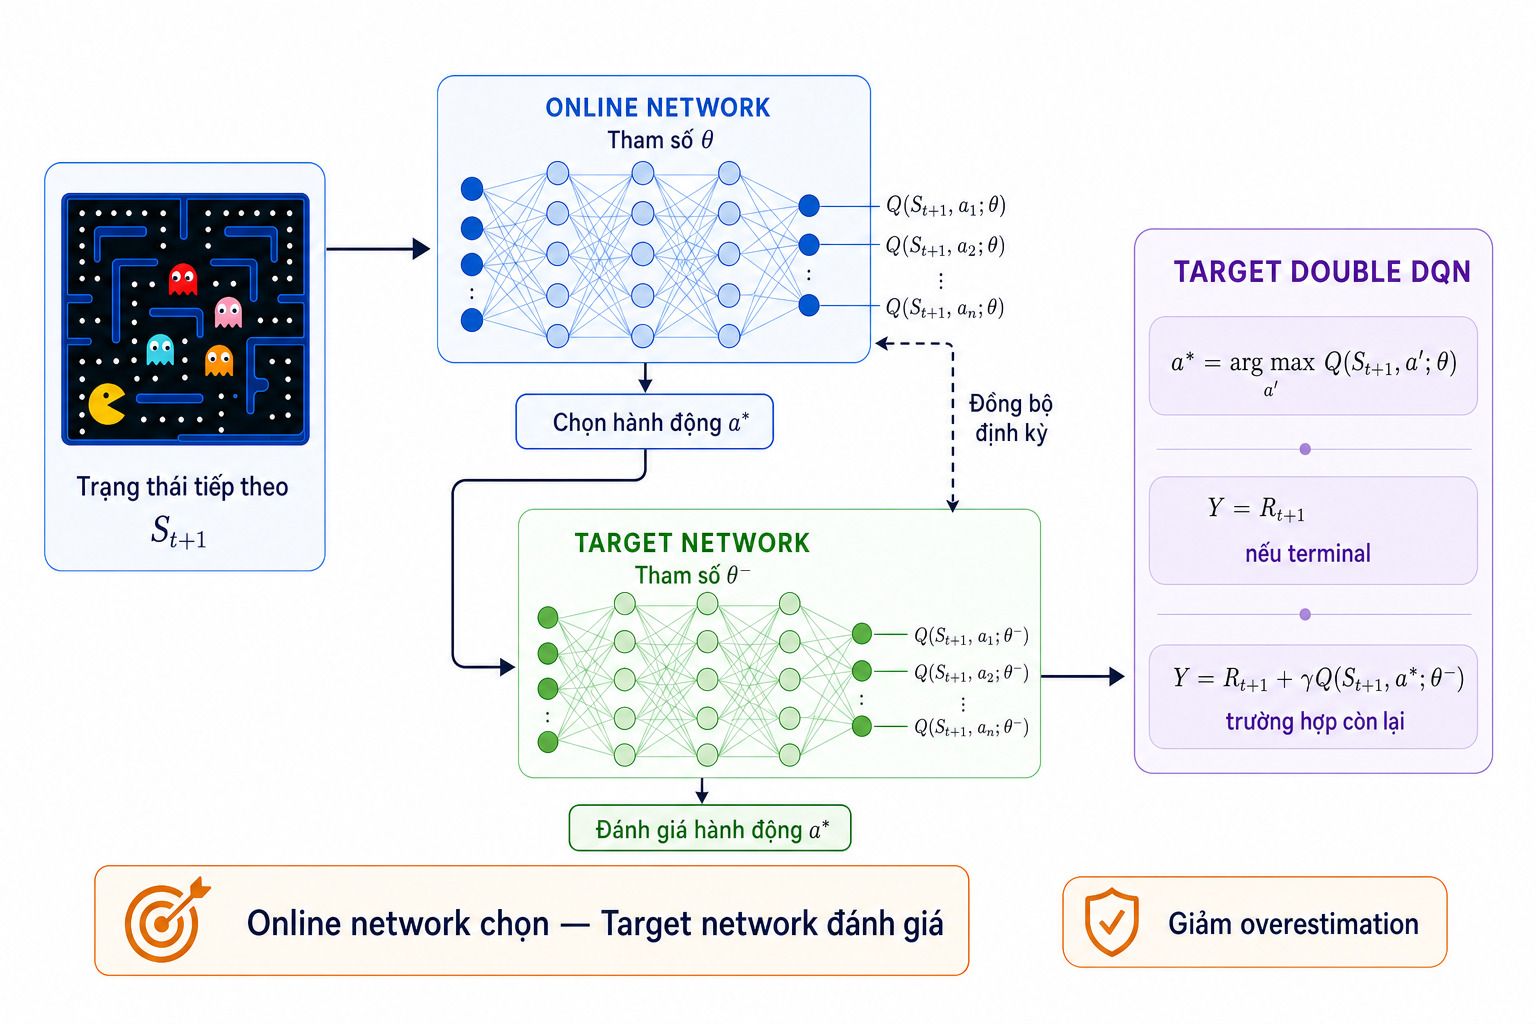
\includegraphics[width=\textwidth]{image/double_dqn_principle.png}
    \caption{Cơ chế lựa chọn và đánh giá hành động khi tính target Double DQN \cite{VanHasselt2016}.}
    \label{fig:ddqn-selection-evaluation}
\end{figure}

Double DQN làm giảm nhưng không loại bỏ hoàn toàn overestimation. Hiệu quả của cơ chế này vẫn phụ thuộc vào dữ liệu, biểu diễn trạng thái, kiến trúc mạng và cấu hình huấn luyện \cite{VanHasselt2016}.

\subsection{So sánh Q-Learning, DQN và Double DQN}

\tabref{tab:algorithm-theory-comparison} tổng hợp những khác biệt quan trọng về nguyên lý của ba thuật toán.

\begin{table}[H]
    \centering
    \renewcommand{\arraystretch}{1.25}
    \small
    \begin{tabular}{@{}
        >{\raggedright\arraybackslash}p{2.7cm}
        >{\raggedright\arraybackslash}p{3.5cm}
        >{\raggedright\arraybackslash}p{3.5cm}
        >{\raggedright\arraybackslash}p{3.5cm}
    @{}}
        \toprule
        \textbf{Tiêu chí} &
        \textbf{Q-Learning} &
        \textbf{DQN} &
        \textbf{Double DQN} \\
        \midrule
        Biểu diễn Q-value &
        Q-table với một phần tử cho mỗi cặp trạng thái--hành động. &
        Mạng Q có tham số $\theta$. &
        Online network và target network như DQN. \\

        Dữ liệu cập nhật &
        Cập nhật trực tiếp từ từng chuyển tiếp. &
        Mini-batch lấy ngẫu nhiên từ replay buffer. &
        Mini-batch lấy ngẫu nhiên từ replay buffer. \\

        Target ở trạng thái tiếp theo &
        Maximum của hàng Q-table tại trạng thái tiếp theo. &
        Target network vừa chọn vừa đánh giá hành động có giá trị lớn nhất. &
        Online network chọn hành động, target network đánh giá hành động đó. \\

        Khái quát hóa &
        Không có cơ chế chia sẻ giá trị giữa các trạng thái khác nhau. &
        Có khả năng chia sẻ thông tin thông qua tham số mạng. &
        Tương tự DQN. \\

        Loss của mạng nơ-ron &
        Không sử dụng. &
        Tối ưu TD error giữa Q-value hiện tại và target DQN. &
        Tối ưu TD error với target Double DQN. \\

        Hạn chế chính &
        Q-table tăng nhanh khi không gian trạng thái lớn. &
        Huấn luyện có thể mất ổn định và xuất hiện overestimation. &
        Giảm overestimation nhưng vẫn phụ thuộc vào hàm xấp xỉ và cấu hình huấn luyện. \\
        \bottomrule
    \end{tabular}
    \caption{So sánh Q-Learning, DQN và Double DQN về mặt nguyên lý.}
    \label{tab:algorithm-theory-comparison}
\end{table}

Q-Learning lưu trực tiếp Q-value trong Q-table. DQN sử dụng mạng nơ-ron để xấp xỉ Q-value, còn Double DQN giữ nguyên cơ chế huấn luyện của DQN nhưng tách quá trình lựa chọn và đánh giá hành động khi tính target.

Từ các cơ sở lý thuyết trên, chương tiếp theo trình bày cách nhóm cụ thể hóa bài toán Mini Pacman thành môi trường học tăng cường, bao gồm biểu diễn trạng thái, không gian hành động, cơ chế phần thưởng và điều kiện kết thúc. Trên nền tảng đó, Q-Learning, DQN và Double DQN được cài đặt trong cùng một hệ thống và đánh giá theo một quy trình thực nghiệm thống nhất.
